\documentclass[a4paper]{scrreprt}
 
\usepackage[german]{babel}
\usepackage[utf8]{inputenc}
\usepackage[T1]{fontenc}
\usepackage{ae}
\usepackage{graphicx}
 \usepackage[bookmarks,bookmarksnumbered]{hyperref}
 
\begin{document}
 
\title{Spielerhandbuch für die Nutzung des Spieles 'Go'}
\author{Harry Flohr (6811837)\\und\\Jan Ole Wellnitz (6796226)}
\maketitle

\tableofcontents 
 
 \chapter{Spielregeln}

Für das Brettspiel GO existieren eine Vielzahl an Regelvarianten (siehe{\url {https://de.wikipedia.org/wiki/Go-Regeln}). Diese GO-Version basiert auf den japanischen Regelwerk mit leichten Varianzen. In den folgenden Absätzen werden die Regeln genauer erklärt. 

\section{Grundlegende Regeln}
\label{sec:Grundlagen}
Das Spiel GO wird von zwei Spielern gespielt, repräsentiert durch die Farben Schwarz und Weiß. Gespielt wird auf einem Gitterfeld aus je neunzehn horizontalen und vertikalen Linien. Die Schnittstellen der Linien sind die bespielbaren Felder, auf denen die Spielsteine gesetzt werden dürfen. Traditionell eröffnet die Farbe Schwarz das Spiel und es wird anschließend abwechselnd ein Spielzug durchgeführt. In seinem Spielzug kann der Spieler einen Stein setzen oder passen. Passen beide Spieler nacheinander wird das Spiel beendet und die Punkte ausgewertet.

\subsection{Vorgabe}
Spielen zwei unterschiedlich starke Spieler gegeneinander kann dem schwächeren Spieler eine Vorgabe gewährt werden. Dabei erhält der schwächere Spieler die Farbe Schwarz und darf zu Spielbeginn eine vorher festgelegte Anzahl an Steinen auf dem Spielfeld verteilen. 

\subsection{Ketten und Freiheiten}
Spielsteine und freie Schnittpunkte auf dem Spielfeld bilden Strukturen mit unterschiedlicher Bedeutung. Über die Gitterlinien verbundene Steine gelten als benachbart. Gleichfarbige benachbarte Steine gelten als Kette. Freiheiten sind leere Schnittpunkte, die an Spielersteine angrenzen. Ein einzelner Spielstein kann bis zu vier Freiheiten haben. \\

\begin{figure}[ht]
\centering \includegraphics[width=0.3\textwidth]{images/freiheit}
\caption{Der schwarze Spielstein hat eine Freiheit, die weißen Steine bilden eine Kette.}
\end{figure}

\newpage

\subsection{Schlagen}
Hat ein Spielstein keine Freiheiten mehr und ist nicht Teil einer Kette, welche Freiheiten hat, gilt er als geschlagen. Somit können auch ganze Ketten geschlagen werden, wenn diese keine Freiheiten mehr teilen. Ein geschlagener Stein wird vom Spielfeld entfernt und als Gefangener gezählt.

\begin{figure}[ht]
\centering \includegraphics[width=0.3\textwidth]{images/schlagen}
\caption{Setzt Weiß einen Stein auf die Markierung verliert die schwarze Kette ihre letzte Freiheit und die vier Steine gelten als geschlagen.}
\end{figure}

\section{Selbstmord und erlaubter Selbstmord}
\label{sec:selbstmord}
Ein Selbstmord liegt vor, wenn ein Stein auf die letzte Freiheit der eigenen Kette gesetzt wird. Dies ist ein ungültiger Zug, außer es werden durch das Setzen gegnerische Steine geschlagen. Werden Steine geschlagen hat die Kette anschließend wieder Freiheiten und es handelte sich um einen "\ erlaubten Selbstmord".

\begin{figure}[ht]
\centering 
\includegraphics[width=0.3\textwidth]{images/selbstmord}
\caption{Setzt Schwarz einen Stein auf die Markierung verliert die schwarze Kette ihre letzte Freiheit. Dies ist ein Selbstmord und damit ein ungültiger Zug.}
\end{figure}

\begin{figure}[ht]
\centering 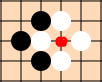
\includegraphics[width=0.3\textwidth]{images/erlaubterselbstmord}
\caption{Setzt Schwarz einen Stein auf die Markierung, hätte dieser keine Freiheiten, aber da durch das Setzen der linke weiße Stein umzingelt und geschlagen ist, bekommt der gesetzte Steine eine Freiheit. Der Zug ist somit gültig.}
\end{figure}
 
\newpage
\section{Auswertung}
\label{sec:Auswertung}
Haben beide Spieler nacheinander gepasst, erfolgt die Auswertung wer gewonnen hat. Die Punktzahl eines Spielers setzt sich zusammen aus der Anzahl der geschlagenen Gegnersteine und der Größe des eroberten Gebiets.\\
Ein Gebiet gilt als erobert, wenn die freien Schnittpunkte von nur einer Farbe umgeben sind. Haben beide Spieler Ketten an einem Gebiet, gilt dieses als neutral und wird nicht gezählt. Gegnersteine, die in einem eroberten Gebiet liegen und kein eigenes Gebiet halten, gelten als geschlagen.\\
Die Anzahl der eroberten Gebiete wird auf die Anzahl der geschlagenen Gegnersteine addiert und der Spieler mit der höheren Punktzahl gewinnt. Bei gleicher Punktzahl gewinnt Weiß. Dies soll den Vorteil ausgleichen den Schwarz durch den ersten Zug hat.

\begin{figure}[ht]
\centering \includegraphics[width=0.3\textwidth]{images/gebiete}
\caption{Schwarz hält ein Gebiet mit vier Punkten, Weiß ein Gebiet mit zwei Punkten und das gemeinsame Gebiet ist neutral.}
\end{figure}

\begin{figure}[ht]
\centering 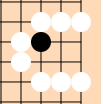
\includegraphics[width=0.3\textwidth]{images/geschlagen}
\caption{Der schwarze Stein liegt innerhalb des weißen Gebiets und hält kein eigenes Gebiet. Er wird bei der Auswertung als geschlagener Stein gezählt.}
\end{figure}

\newpage

\chapter {Spielen mit der Software}
\section{Bedienung der Software}
Die Software wird mit Maus und Tastatur bedient, wobei die Tastatur nur zur Eingabe von Zahlen benötigt wird. Wird der Spieler zur Eingabe von Zahlen aufgefordert, werden die Nummerntasten 0-9 zur Eingabe, die Entertaste zur Bestätigung und die Backspacetaste zur Korrektur benötigt. Anonsten wird das Programm über Mausklick gesteuert.

\section {Start der Software}
\label{sec:start}
Um die Software zu starten wird zuerst der Server benötigt. Dieser wird über den Pfad go\textbackslash{}src\textbackslash{}go\_server.rkt  gestartet und einfach ausgeführt.
Dies startet das Universum, welches anschließend auf die Anmeldung von zwei Clients wartet.\\\\

Die Clients werden über den Pfad go\textbackslash{}src\textbackslash{}go\_client.rkt gestartet. Wird der Client ausgeführt, werden zwei Instanzen gestartet, welche sich am lokalen Server anmelden. Der Client, der sich als erstes anmeldet, erhält einige Auswahlmöglichkeiten zum Spielstart.\\
Die erste Wahl ist die Art des Spielstarts. Hier steht zur Auswahl ob ein neues Spiel begonnen werden soll oder ein Spiel über ein Bild eingelesen werden soll.


\section{Start eines neuen Spiel}
Wird ein neues Spiel als Spielstart ausgewählt, hat der Spieler einige Eingaben zu wählen:

\begin{enumerate}
\item Wahl der Farbe:\\
Der Spieler wählt ob er als Schwarz oder Weiß spielt, sein Gegenspieler erhält die andere Farbe.

\item Wahl der Vorgabe:\\
Der Spieler wählt ob Schwarz mit einer Vorgabe anfängt. Dabei wird die Höhe über die Nummerntasten eingegeben, Korrekturen erfolgen über Backspace und mit Enter wird die Eingabe bestätigt.

\item Setzen der Vorgabe:\\
Wurde eine Vorgabe gewählt, darf Schwarz Spielsteine in Höhe der Vorgabe auf das Spielfeld setzen.Gesetzt wird durch anklicken des Schnittpunkts auf den der Stein gesetzt werden soll. Anschließend beginnt das Spiel.

\end{enumerate}

\begin{figure}[ht]
\centering 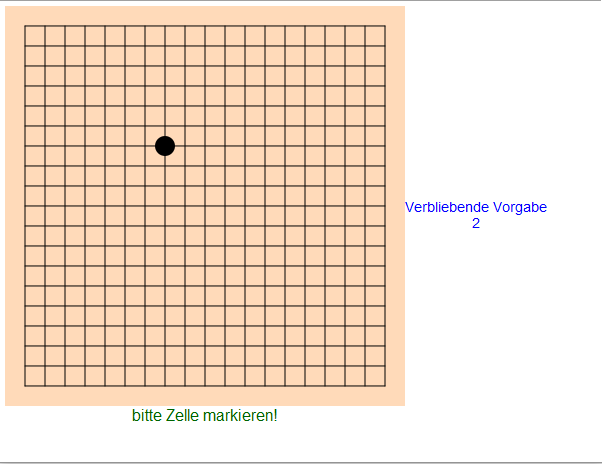
\includegraphics[width=1.0\textwidth]{images/Vorgabe}
\caption{Schwarz setzt seine Vorgabe. Die verbleibenden Steine der Vorgabe werden rechts vom Spielfeld angezeigt.}
\end{figure}

\section{Start eines Spiels aus einem Bild}
\subsection{Anforderungen an das Bild}
Um ein Spielfeld als Bild in die Software einlesen zu können, muss das Bild einige Anforderungen erfüllen:

\begin{enumerate}
\item Art des Spielbretts:
Es Sollte sich um ein typisches GO-Turnierbrett handeln. Bei diesen entspricht der Abstand von den äußeren Gitterpunkten bis zum Rand genau die Hälfte des Abstandes zwischen den einzelnen Gitterpunkten.

\item Aufnahmewinkel:
Die Aufnahme sollte senkrecht von oben erfolgen und das Spielfeld muss rechtwinklig im Bild liegen. Ein ausreichender Abstand zum Spielfeld bei der Aufnahme ist empfehlenswert um mögliche Verzerrungen durch das Objektiv zu minimieren.

\item Beleuchtung:
Das Spielfeld sollte gleichmäßig ausgeleuchtet sein. Starke direkte Beleuchtung vermeiden, um Spiegelungen auf dem Spielfeld zu minimieren.
\end{enumerate}

\begin{figure}[ht]
\centering 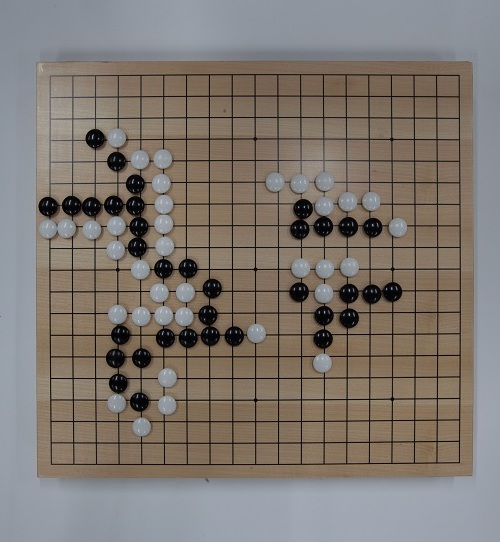
\includegraphics[width=0.8\textwidth]{images/Spielbrett}
\caption{Beispielaufnahme. Das Spielfeld hat die richtige Ausrichtung. Die Spiegelungen sind das Maximum, welches die Software verarbeiten kann.}
\end{figure}

\newpage 

\subsection{Speicherort und Einlesen des Bildes}
Das Bild wird im Pfad  go\textbackslash{}images\textbackslash{} gespeichert. Der Name des Bilds aus eingelesen werden soll, muss in  go\textbackslash{}src\textbackslash{}go\_bv.rkt im markierten Bereich eingetragen werden.\\
 Eine Änderung des Bildes ist nur möglich, wenn der Server nicht läuft. Dazu sollte der go\_server vollständig gestoppt und neu gestartet werden.
\begin{figure}[ht]
\centering 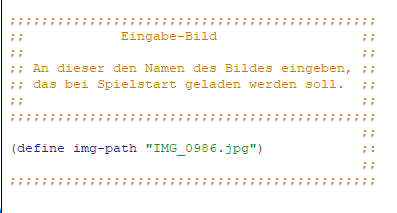
\includegraphics[width=0.8\textwidth]{images/Bildname}
\caption{Hier wird in go\_bv.rkt der Name des Bildes eingetragen.}
\end{figure}

Anschließend wird das Bild automatisch eingelesen, wenn ein Start aus einer Bilddatei ausgewählt wurde.

\subsection{Auswahlmöglichkeiten beim Start aus einer Bilddatei}
Beim Einlesen eines Spielstandes aus einer Bilddatei benötigt der Server noch mehrere Informationen bevor gespielt werden kann:

\begin{enumerate}
\item Eingabe der geschlagenen Steine:\\
Der Spieler gibt an wie viele Steine bereits geschlagen wurden. Dabei wird die Höhe über die Nummerntasten eingegeben, Korrekturen erfolgen über Backspace und mit Enter wird die Eingabe bestätigt.

\item Wahl der Farbe:\\
Der Spieler wählt ob er als Schwarz oder Weiß spielt, sein Gegenspieler erhält die andere Farbe.

\item Passstatus:\\
Der Spieler gibt an ob vor der Aufnahme gepasst wurde. 

\item Zugreihenfolge:\\
Der Spieler gibt an welche Farbe als nächstes setzen darf. Anschließend beginnt das Spiel.
\end{enumerate}

\newpage

\section {Spielen}

Wurde ein Spielstart gewählt und alle Eingaben getätigt, kann gespielt werden. Der Client zeigt das Spielfeld an. Rechts vom Spielfeld werden die geschlagenen Steine mitgezählt und unter dem Spielfeld steht wer gerade setzen darf und ob im vorherigen Zug gepasst wurde.\\
Ein Zug erfolgt wenn ein Stein durch Klicken in das Spielfeld gesetzt wurde oder gepasst wird durch betätigen des "\ Passen" Buttons.\\
Falls ein Spieler einen ungültigen Zug durchführen möchte, kann der Stein nicht gesetzt werden.

\begin{figure}[ht]
\centering 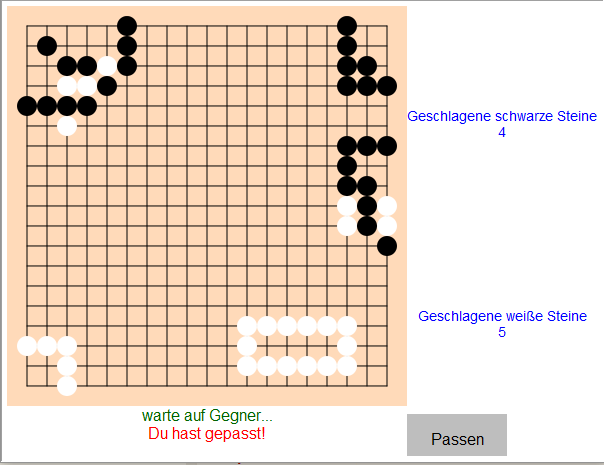
\includegraphics[width=0.8\textwidth]{images/spielen}
\caption{Client-Sicht. Der andere Spieler ist zur Zeit am Zug und es wurde im vorherigen Zug gepasst.}
\end{figure}

\newpage

\section{Auswertung)}
Haben beide Spieler nacheinander gepasst, erscheint die Auswertung. Rechts vom Spielfeld werden die finalen Punkte angezeigt, welche sich aus der Anzahl der geschlagenen Gegnersteine und der eroberten Gebiete zusammensetzt. Unter dem Spielfeld wird angezeigt wer gewonnen hat.\\
Es kann ein neues Spiel gestartet werden, wenn der Button "\  Neues Spiel"\ von einem der Spieler betätigt wird.

\begin{figure}[ht]
\centering 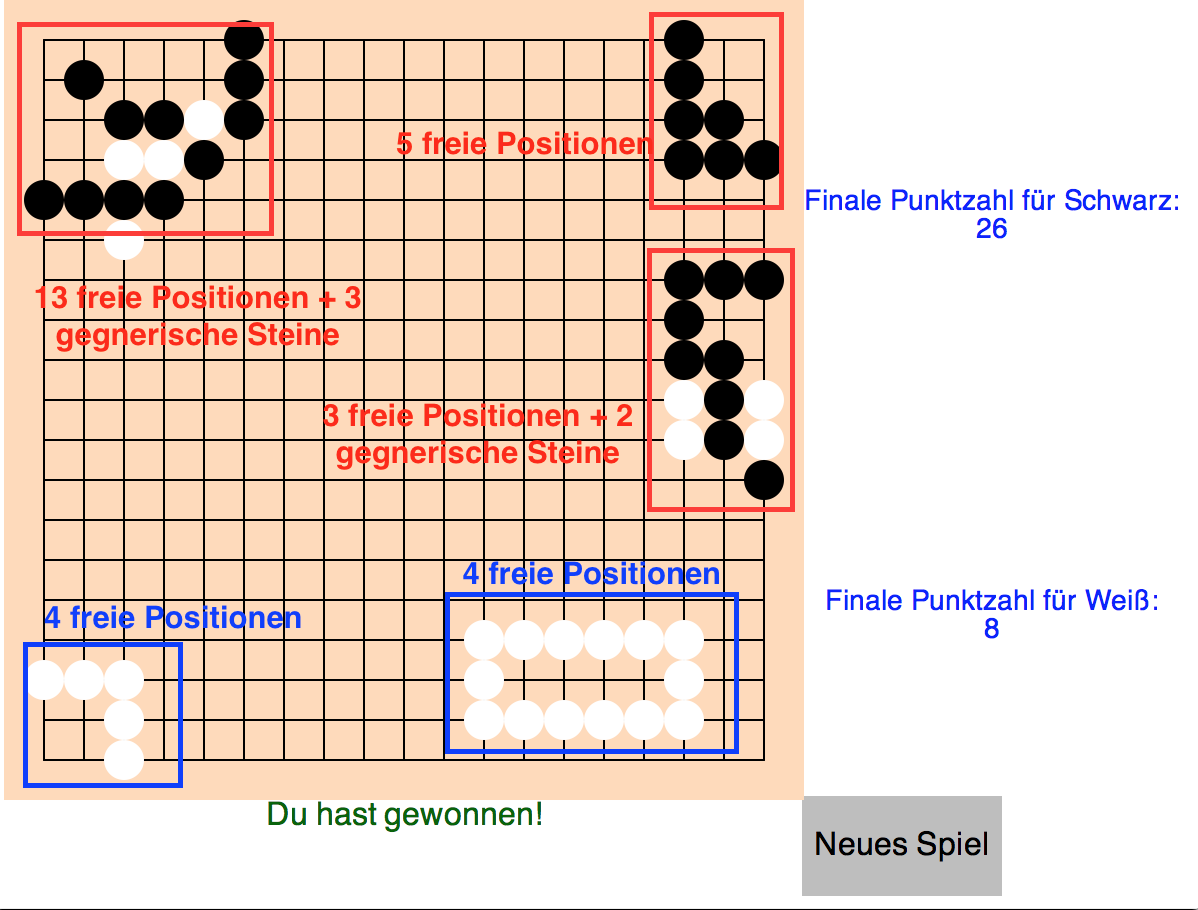
\includegraphics[width=0.8\textwidth]{images/auswertung}
\caption{In diesem Beispiel hat Schwarz gewonnen.}
\end{figure}




\end{document}
